\documentclass[16pt]{report}

\usepackage{graphicx}
\usepackage[utf8]{inputenc}
\usepackage[spanish]{babel}

% citas:
%\usepackage{cite}
\usepackage[numbers]{natbib}
\usepackage{url}


\begin{document}
%Portada
\begin{titlepage}
	\centering
	{
\includegraphics[width=0.2\textwidth]{pictures/Universidad_Veracruzana}\par}
	\vspace{1cm}
	{\bfseries\LARGE Universidad Veracruzana \par}
	\vspace{1cm}
	{\scshape\Large Ingeniería Biomédica \par}
	\vspace{3cm}
	{\scshape\Huge Interfaz para un filtro de frecuencia cardiáca. \par}
	\vspace{2cm}
	{\itshape\Large Proyecto. \par}
	\vfill
	{\Large Autores: \par}
	{\Large Caballero Trinidad Flor Isabel. \\ Cortés Ramírez Samuel Jefte. \\ García García Ian Pablo. \\ Pérez Roldan Eduardo Alejandro. \\ Cabañas Alba Alejandro. \\ Alfonso Gamboa Rubén. \par}
	\vfill
\end{titlepage}


% Cuerpo del reporte
\chapter{Parcial 2}
\section{keywords}
Frecuencia cardaica, Interfaz, Filtro de frecuencia cardaiaca, Interfaz para un filtro, SPython, Interfaz Médica, Ingeniería Biomédica, Arduino.

\section{Introducción.}
El siguiente proyecto tiene como finalidad responder a la pregunta ¿Cómo desarrollar una interfaz que facilite la visualización y procesamiento de datos de la frecuencia cardiaca?, teniendo como principal objetivo visualizar la frecuencia cardiaca del usuario mediante una interfaz a partir del lenguaje de programación Python \cite{python}. 

Los temas que se abordaran y se trabajaran para la realización óptima del proyecto son: desarrollar una interfaz amigable con el usuario con la finalidad de interpretar los datos de manera precisa, garantizando la funcionalidad del sistema diseñando una interfaz para una gráfica; con el lenguaje de programación Python. Se busca leer y escribir ficheros, desarrollar un código legible para el programador y una forma de almacenar los datos recolectados, con el propósito de calcular la media aritmética para añadir funcionalidad que permita al usuario calcular su recuperación cardiaca. Este proyecto esta dirigido a un público general busca monitorear su frecuencia cardiaca.  

Se llevará a cabo el proyecto con la finalidad de adquirir conocimiento sobre la creación de una interfaz en el lenguaje de programación Python, con la ayuda de una practica anterior relacionada a la Ingeniería Biomédica, se obtendrán lecturas de medición para la realización de prueba predictiva en índices para medir la salud cardiaca, se diseñara una versión base de una interfaz para el almacenamiento de señales biomédicas, con la finalidad de utilizarlas en un futuro y poder manipularlas, también se trabajara en conjunto con compañeros de la carrera de Instrumentación Electrónica, para así reforzar el trabajo en equipo y crear un frontend y un backend. 

Para filtrar la búsqueda de la información necesaria para poder realizar el proyecto, se procedió a una búsqueda sistematizada de evidencia siguiendo los criterios de inclusión: artículos, libros, tesis, publicadas desde el año 1990 hasta la actualidad, información relacionada a como crear una interfaz en el lenguaje de programación Python, información del funcionamiento y características de la frecuencia cardiaca. 

En esta sección se elabora una revisión bibliográfica de los conceptos generales a partir de los cuales se sustenta este proyecto, los conceptos a considerar son: señales biomédicas, interfaz, base de datos, frontend, backend, lenguaje de programación Python, frecuencia cardiaca.

\paragraph{Señales biomédicas.} ¿Qué es una señal biomédica? "Las señales biomédicas representan variables fisiológicamente relevantes de las que nos interesa su curso temporal. La variable puede ser un voltaje muy pequeño, como el electroencefalograma, o algunos órdenes de magnitud mayor, como el electrocardiograma, o puede ser una variable que originalmente no es eléctrica, como la presión o la temperatura" \cite{biomedica_s}. 
\paragraph{Interfaz.} ¿Qué es una interfaz? la RAE la define como: "Conexión o frontera común entre dos aparatos o sistemas independientes, quepermite el intercambio de información o la coordinación de sus funciones." \cite{rae_interfaz}
\paragraph{Frontend y backend.} ¿Qué es front-end y back-end?. El front-end es la parte que va a interactuar con el usuario, en el caso de nuestroproyecto será la interfaz, el back-end es la parte que contiene la infraestructura quele va a dar funcionalidad a el proyecto. \cite{FrontendBackend}
\paragraph{Lenguaje de programación Python.} Python es un lenguaje de progamación de alto nivel, el cual ha agarrado bastante popularidad en nuestros tiempos gracias a su legibilidad, razón por la cual también es el más usado en cuanto a aprender a programar se refiere; razón por la cual hoy en dia contamos con un sin fin de librerías y documentación al respecto. \cite{python}
\paragraph{Frecuencia cardiaca.} La frecuencia cardiaca o pulso, es la cantidad de veces que late por cierto periodode tiempo, se puede medir en varias partes del cuerpo como la muñeca, cuello,pecho, entre otros. La frecuencia de un adulto suele encontrarse dentro de 60 – 100latidos por minuto.\cite{FrecuenciaCardiaca}

\section{Metodología.}
Se utilizará el lenguaje de programación Python \cite{python} para la aplicación principal. Se utilizará la librería “TkInter”\cite{tkinter} y la librería "Custom TkInter" \cite{customtkinter} para el diseño de una interfaz "amigable" con el usuario.\\
Para el despliegue de las gráficas de pulso cardiaco se utilizará la librería matplotlib \cite{matplotlib}. \\
Para la obtención de las señales cardiacas se utilizará un sensor "Max 30100” (figura \ref{sensor}) y una placa arduino uno (figura \ref{arduino}) con el cual se medirá el pulso cardiaco de una persona; para la comunicación se utilizara un programa por aparte heco en python. Posteriormente guardarlo en un archivo “csv", dicho archivo pasará por un filtro realizado por nuestros compañeros de instrumentación electrónica para así entregarnos una señal legible y más limpia; para posteriormente ser gráficada en nuestra aplicación.\\
Para una mejor organización y para un control se versiones, se usará git y github. Publicado en: https://github.com/Benchito2003/Proyecto-programacion.git.

\begin{figure}[h]
	\caption{Placa arduino uno}
	\centering
	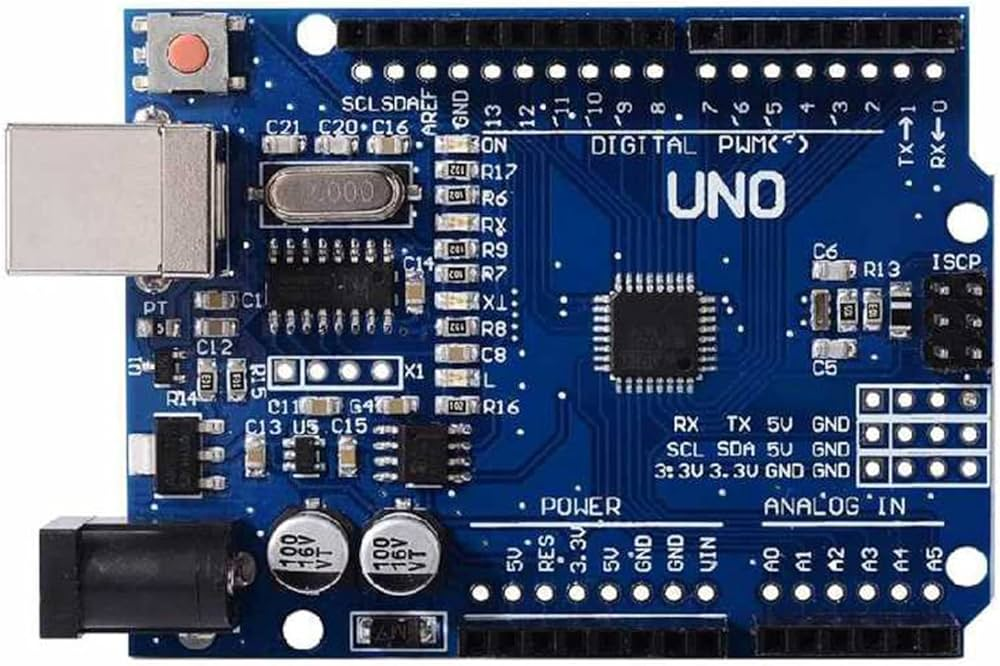
\includegraphics[width=0.5\textwidth]{pictures/placa-arduino}
	\label{arduino}
\end{figure}


\begin{figure}[h]
	\caption{Sensor max 30100}
	\centering
	
\includegraphics[width=0.5\textwidth]{pictures/imagen}
	\label{sensor}
\end{figure}

\subsection{Funcionamiento del código} El código se empezó a programar con ayuda de la programación orientada a objetos, donde cada ventana, frame o widget es en realidad una clase (o molde) hecho por nosotros, de manera que simplemente los mandamos a llamar, algunas carácterísticas generales de estas clases son: que comparten la misma paleta de colores, comparten la misma fuente, sus módulos pueden ser ejecutados ahí mismo para testear que dicho módulo esté funcionando correctamente. \\
Para ésto, la documentacón de Custom Tkinter \cite{customtkinter}, cuenta con varios ejemplos ilustrativos de como podemos trabajar con sus clases orientadas a objetos, por lo que nosotros lo que lo unico que se ralizó fue heredar de éstas clases sus métodos y características (osease heredados).
\subsubsection{colores}
Figura: \ref{colores}. Primeramente se hicieron varios conjuntos de colores en forma de listas, para poder escoger a futuro, el color que le quedaría mejor a nuestra interfaz, pudiendo establecer desde un principio la paleta con la que iremos trabajando.
\begin{figure}[h!]
	\caption{módulo "colores.py"}
	\centering
	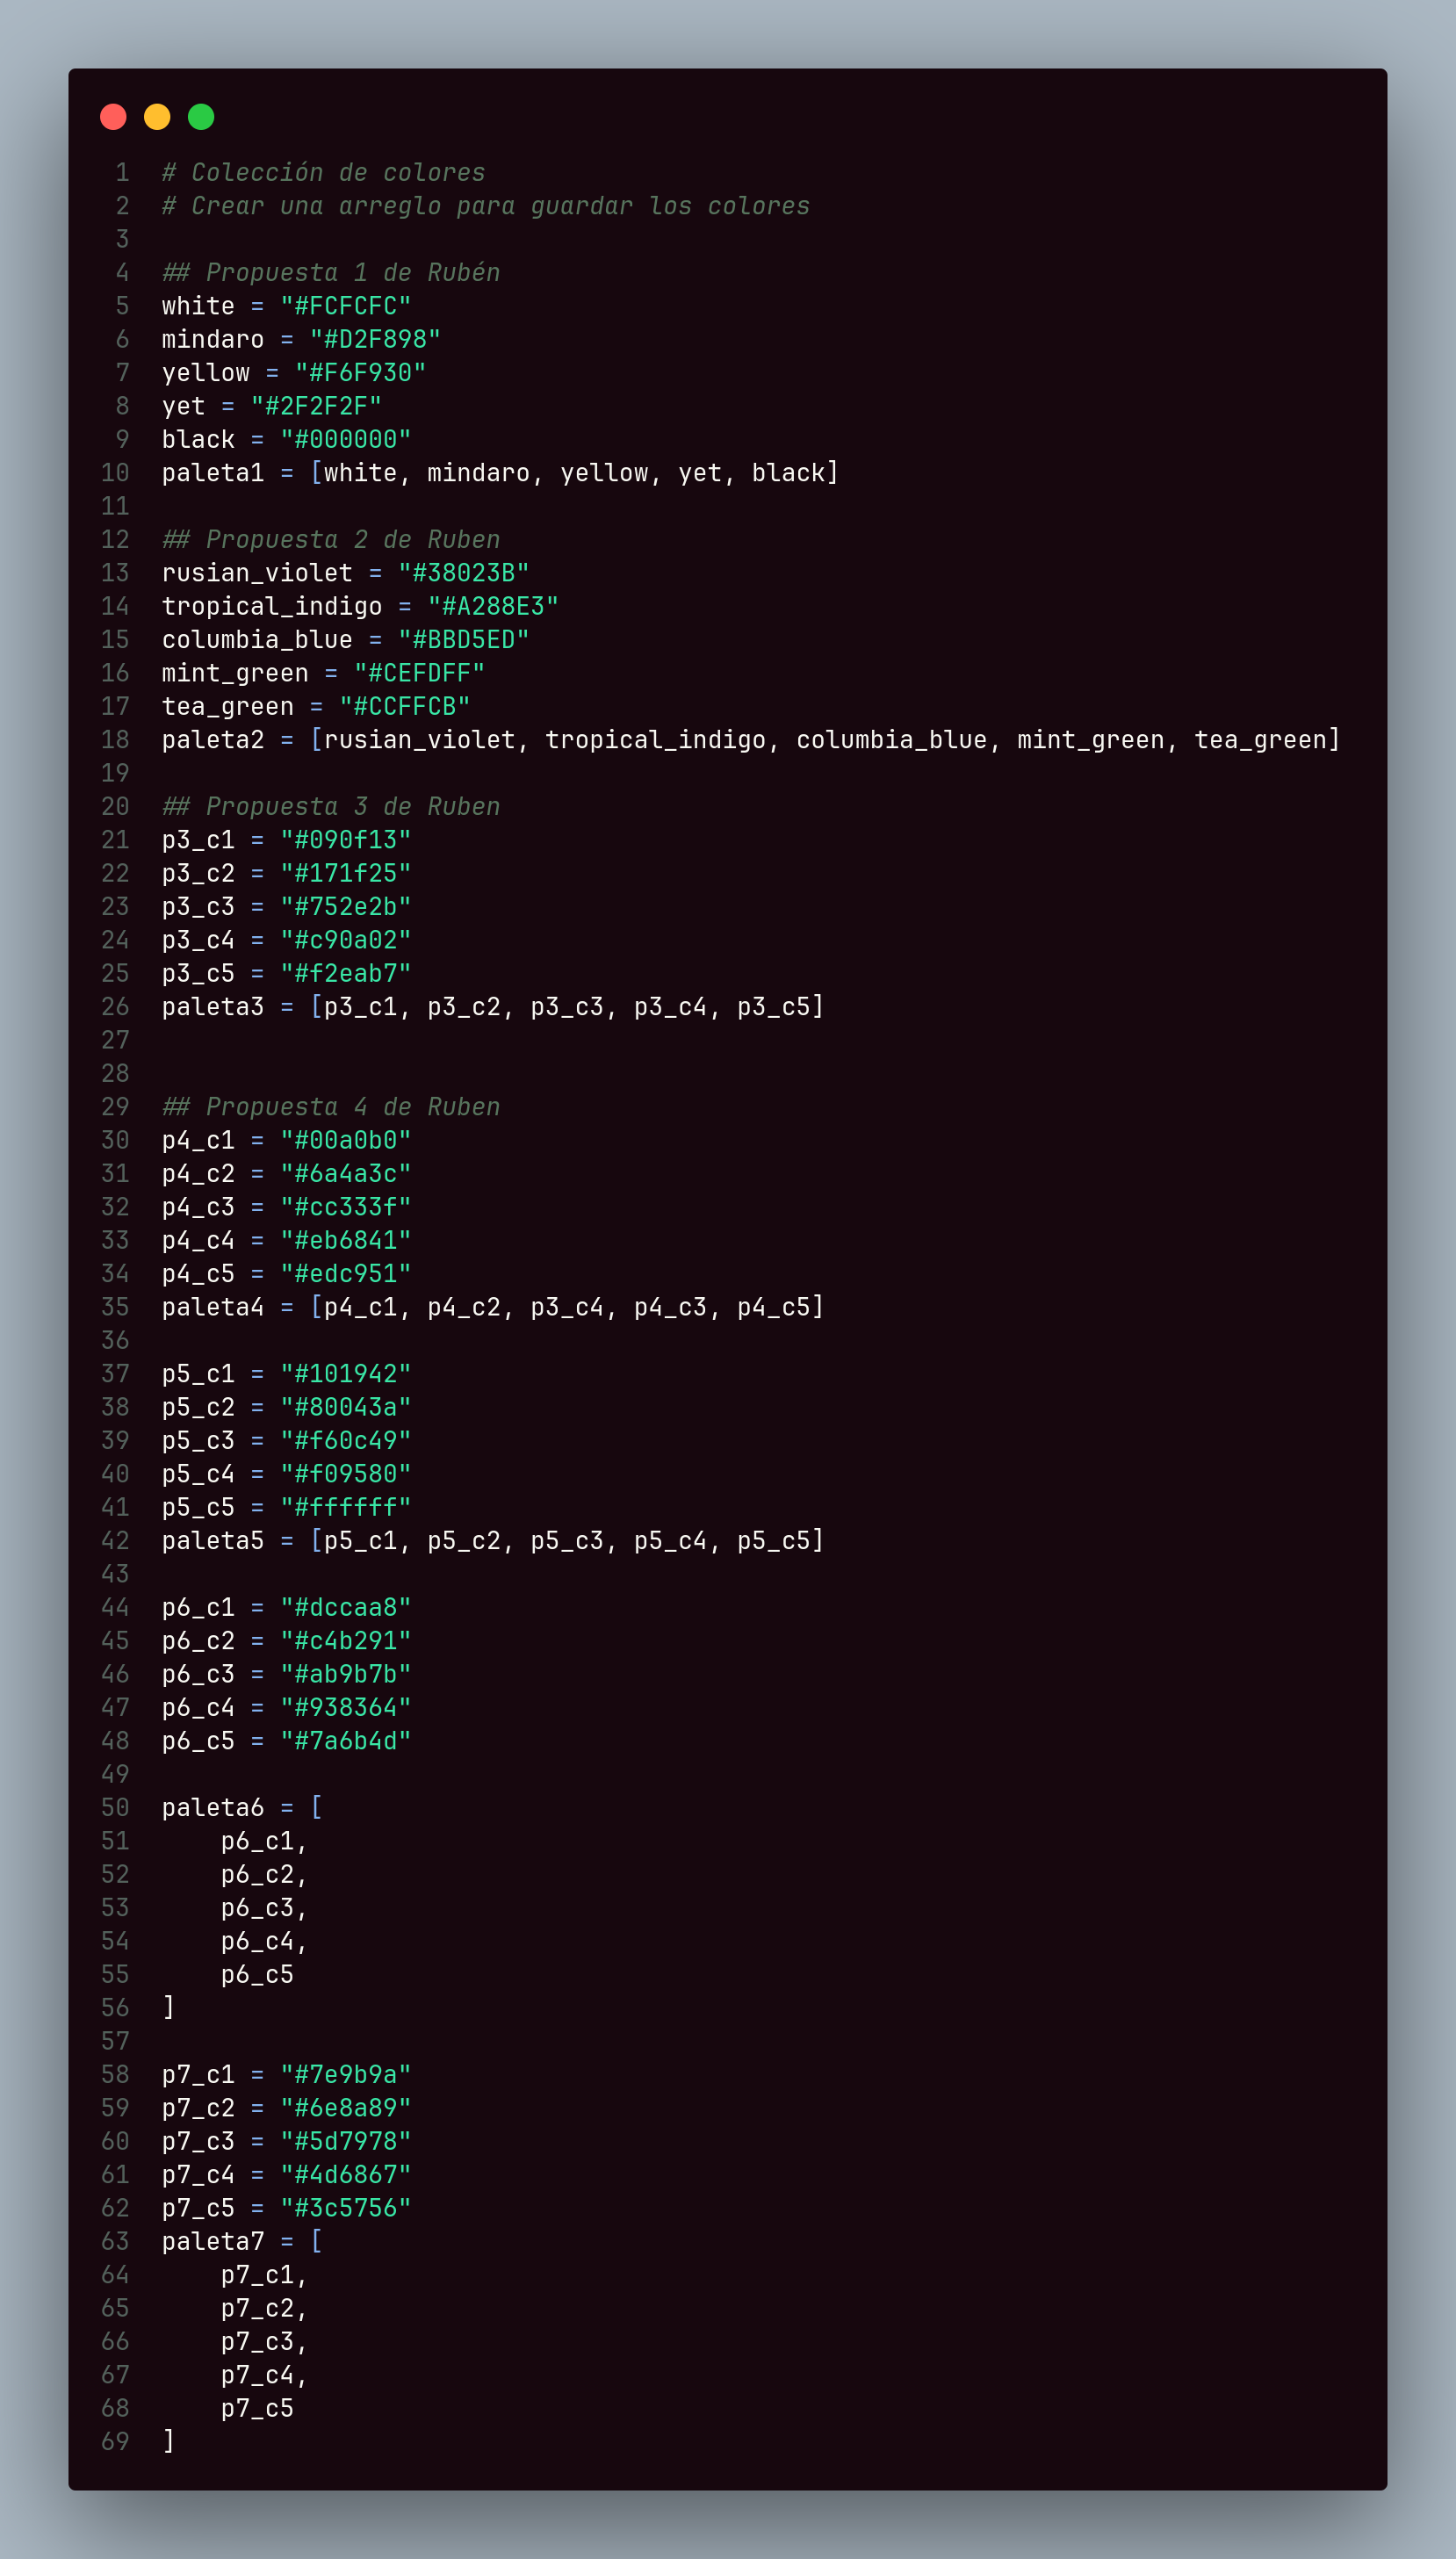
\includegraphics[width=1\textwidth]{pictures/capturas/colores}
	\label{colores}
\end{figure}

\subsubsection{config}
Importamos custom tkinter \cite{customtkinter} \\
El módulo config (figura \ref{config}) es un módulo donde creamos clases o moldes para nuestros botones, etiquetas, entre otros; dejando que hereden lo importante de custom tkinter \cite{customtkinter} y después asignandoles nuestros propios "Valores por defecto". Les asignamos colores acorde a la paleta de colores asiganada y ya están listos para ser usados por el resto del programa. Así se ahorra el repetir bastante código, y en caso de ser necesario un cambio hacia todas las etiquetas, se puede hacer directamente desde este módulo. 

\begin{figure}[h!]
	\caption{Módulo "config.py"}
	\centering
	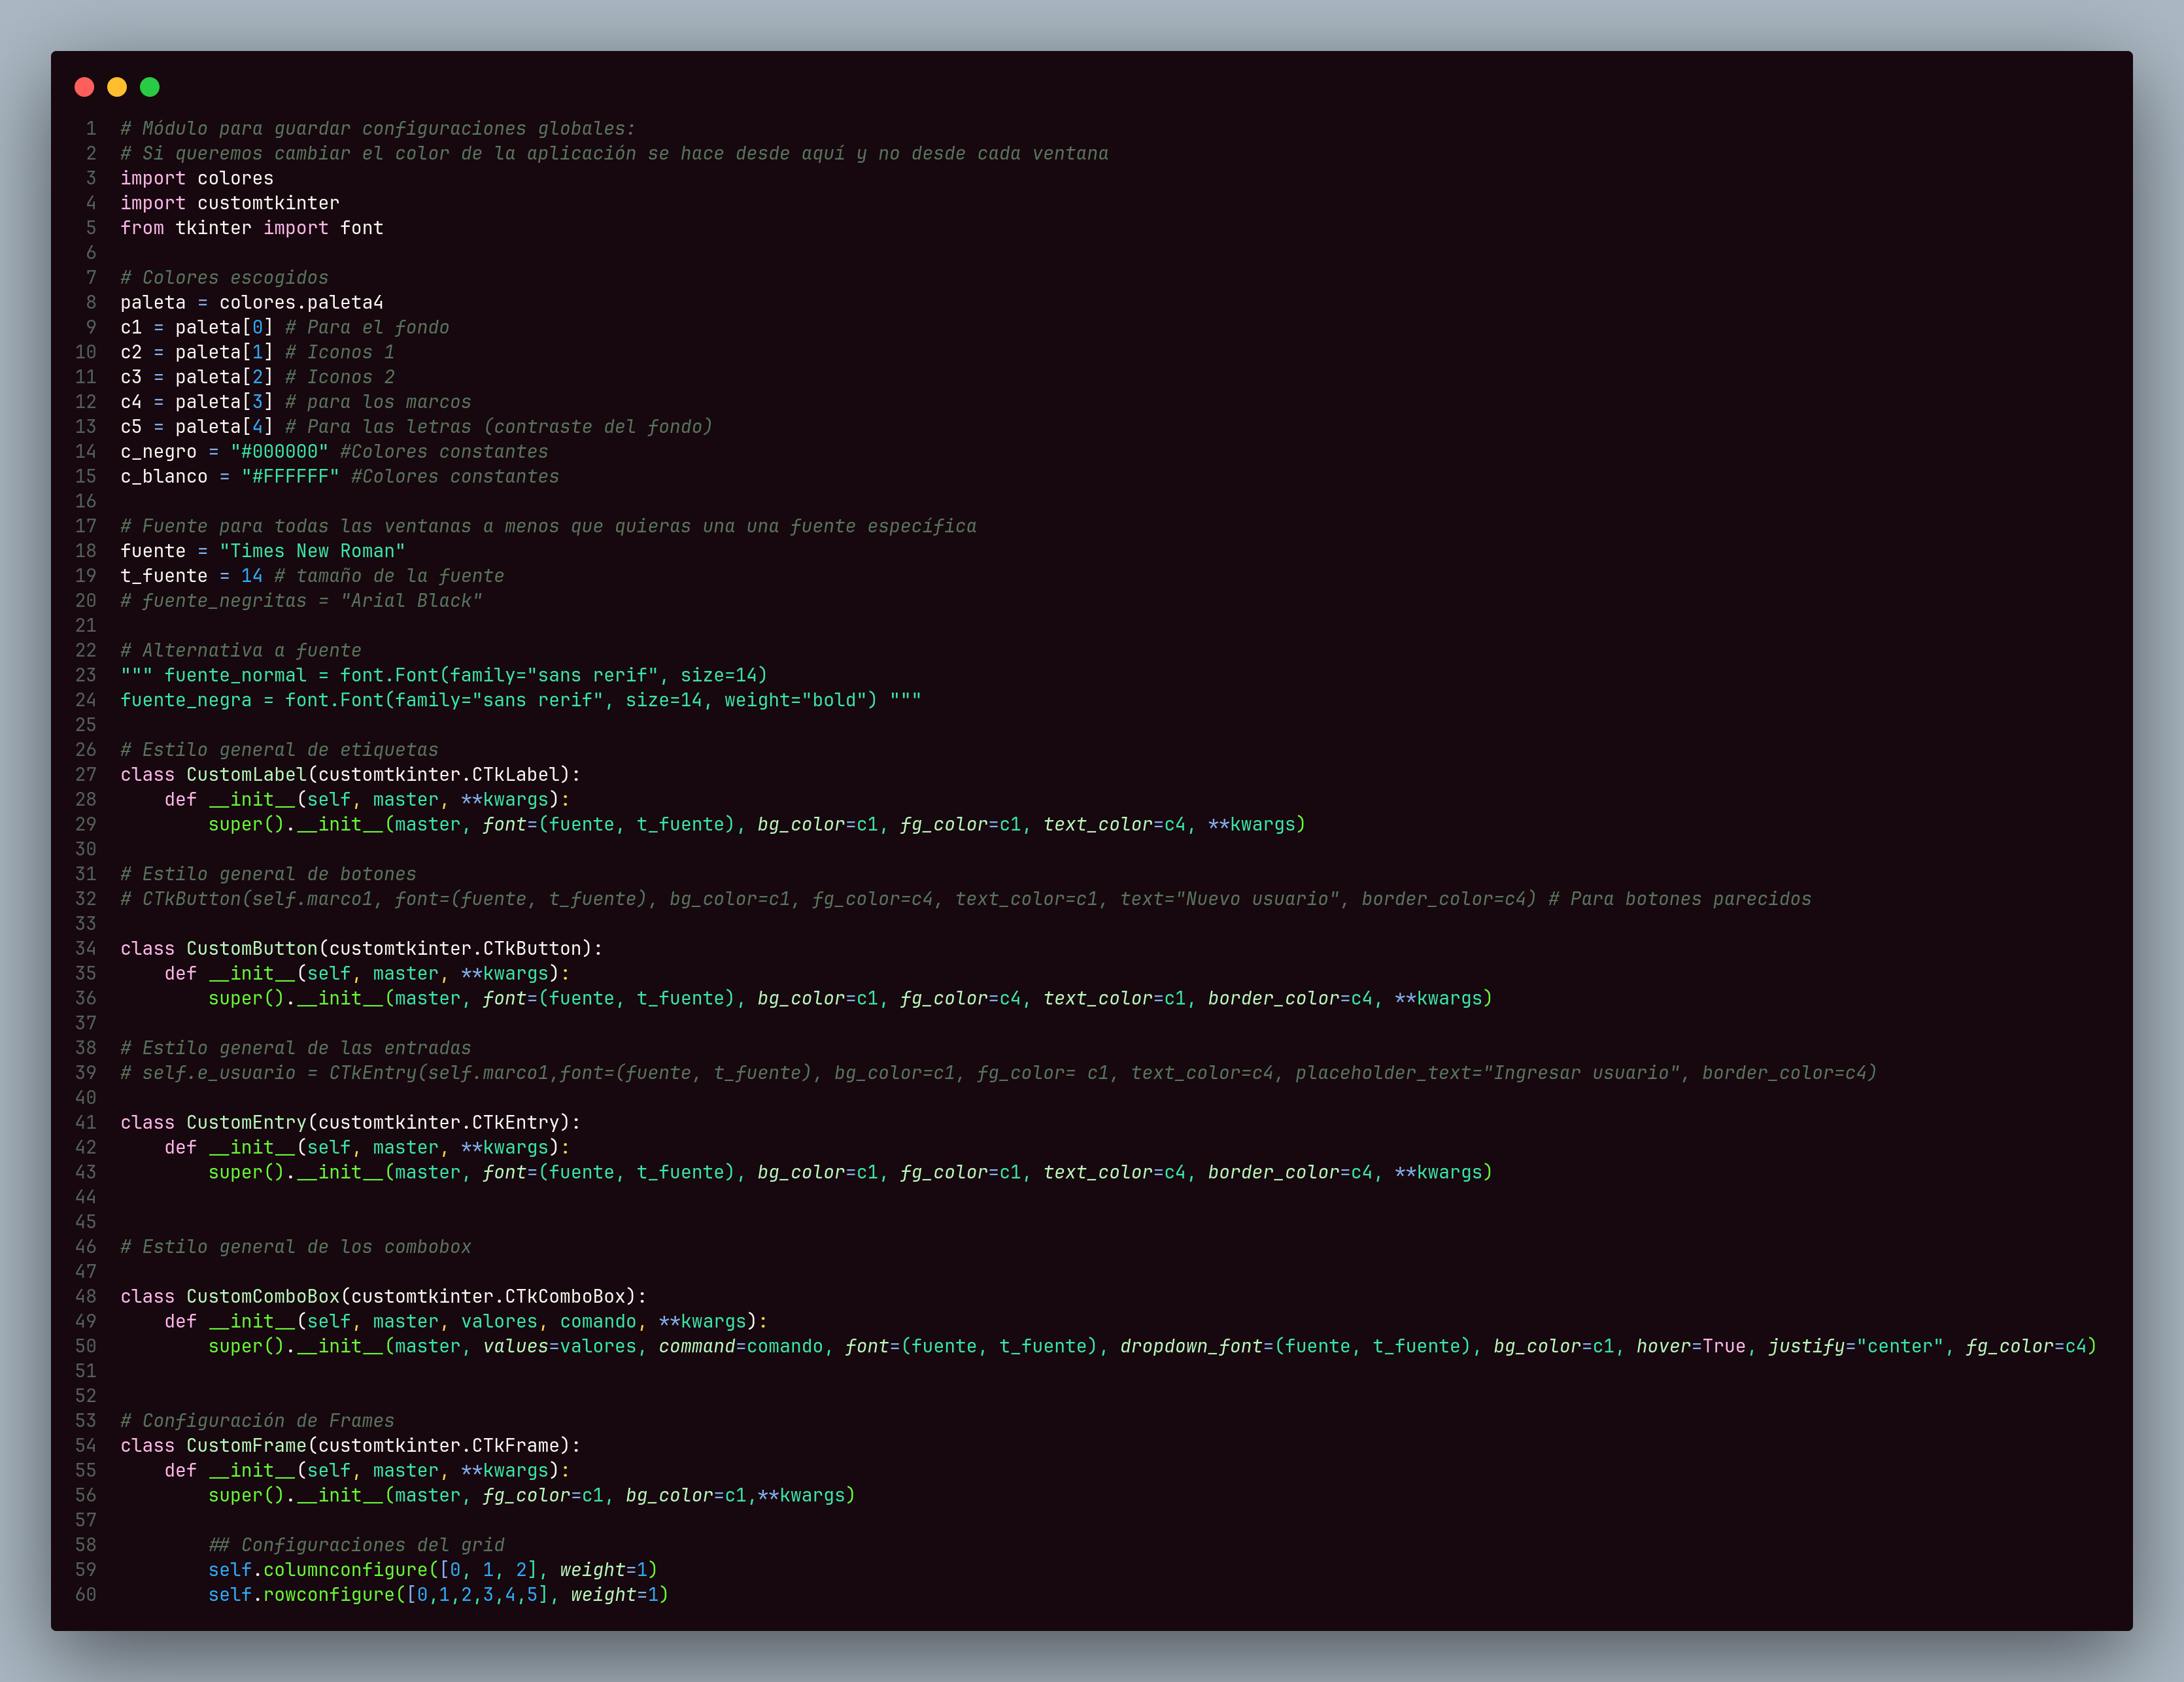
\includegraphics[width=1\textwidth]{pictures/capturas/config}
	\label{config}
\end{figure}

\subsubsection{Frames}
Para la construcción de cada frame (figura \ref{frames}), solo se llama desde el modulo de config a clase, siguiendo el ejemplo de la documentación de custom tkinter \cite{customtkinter}

\begin{figure}[h!]
	\caption{Ejemplo de creación de un frame}
	\centering
	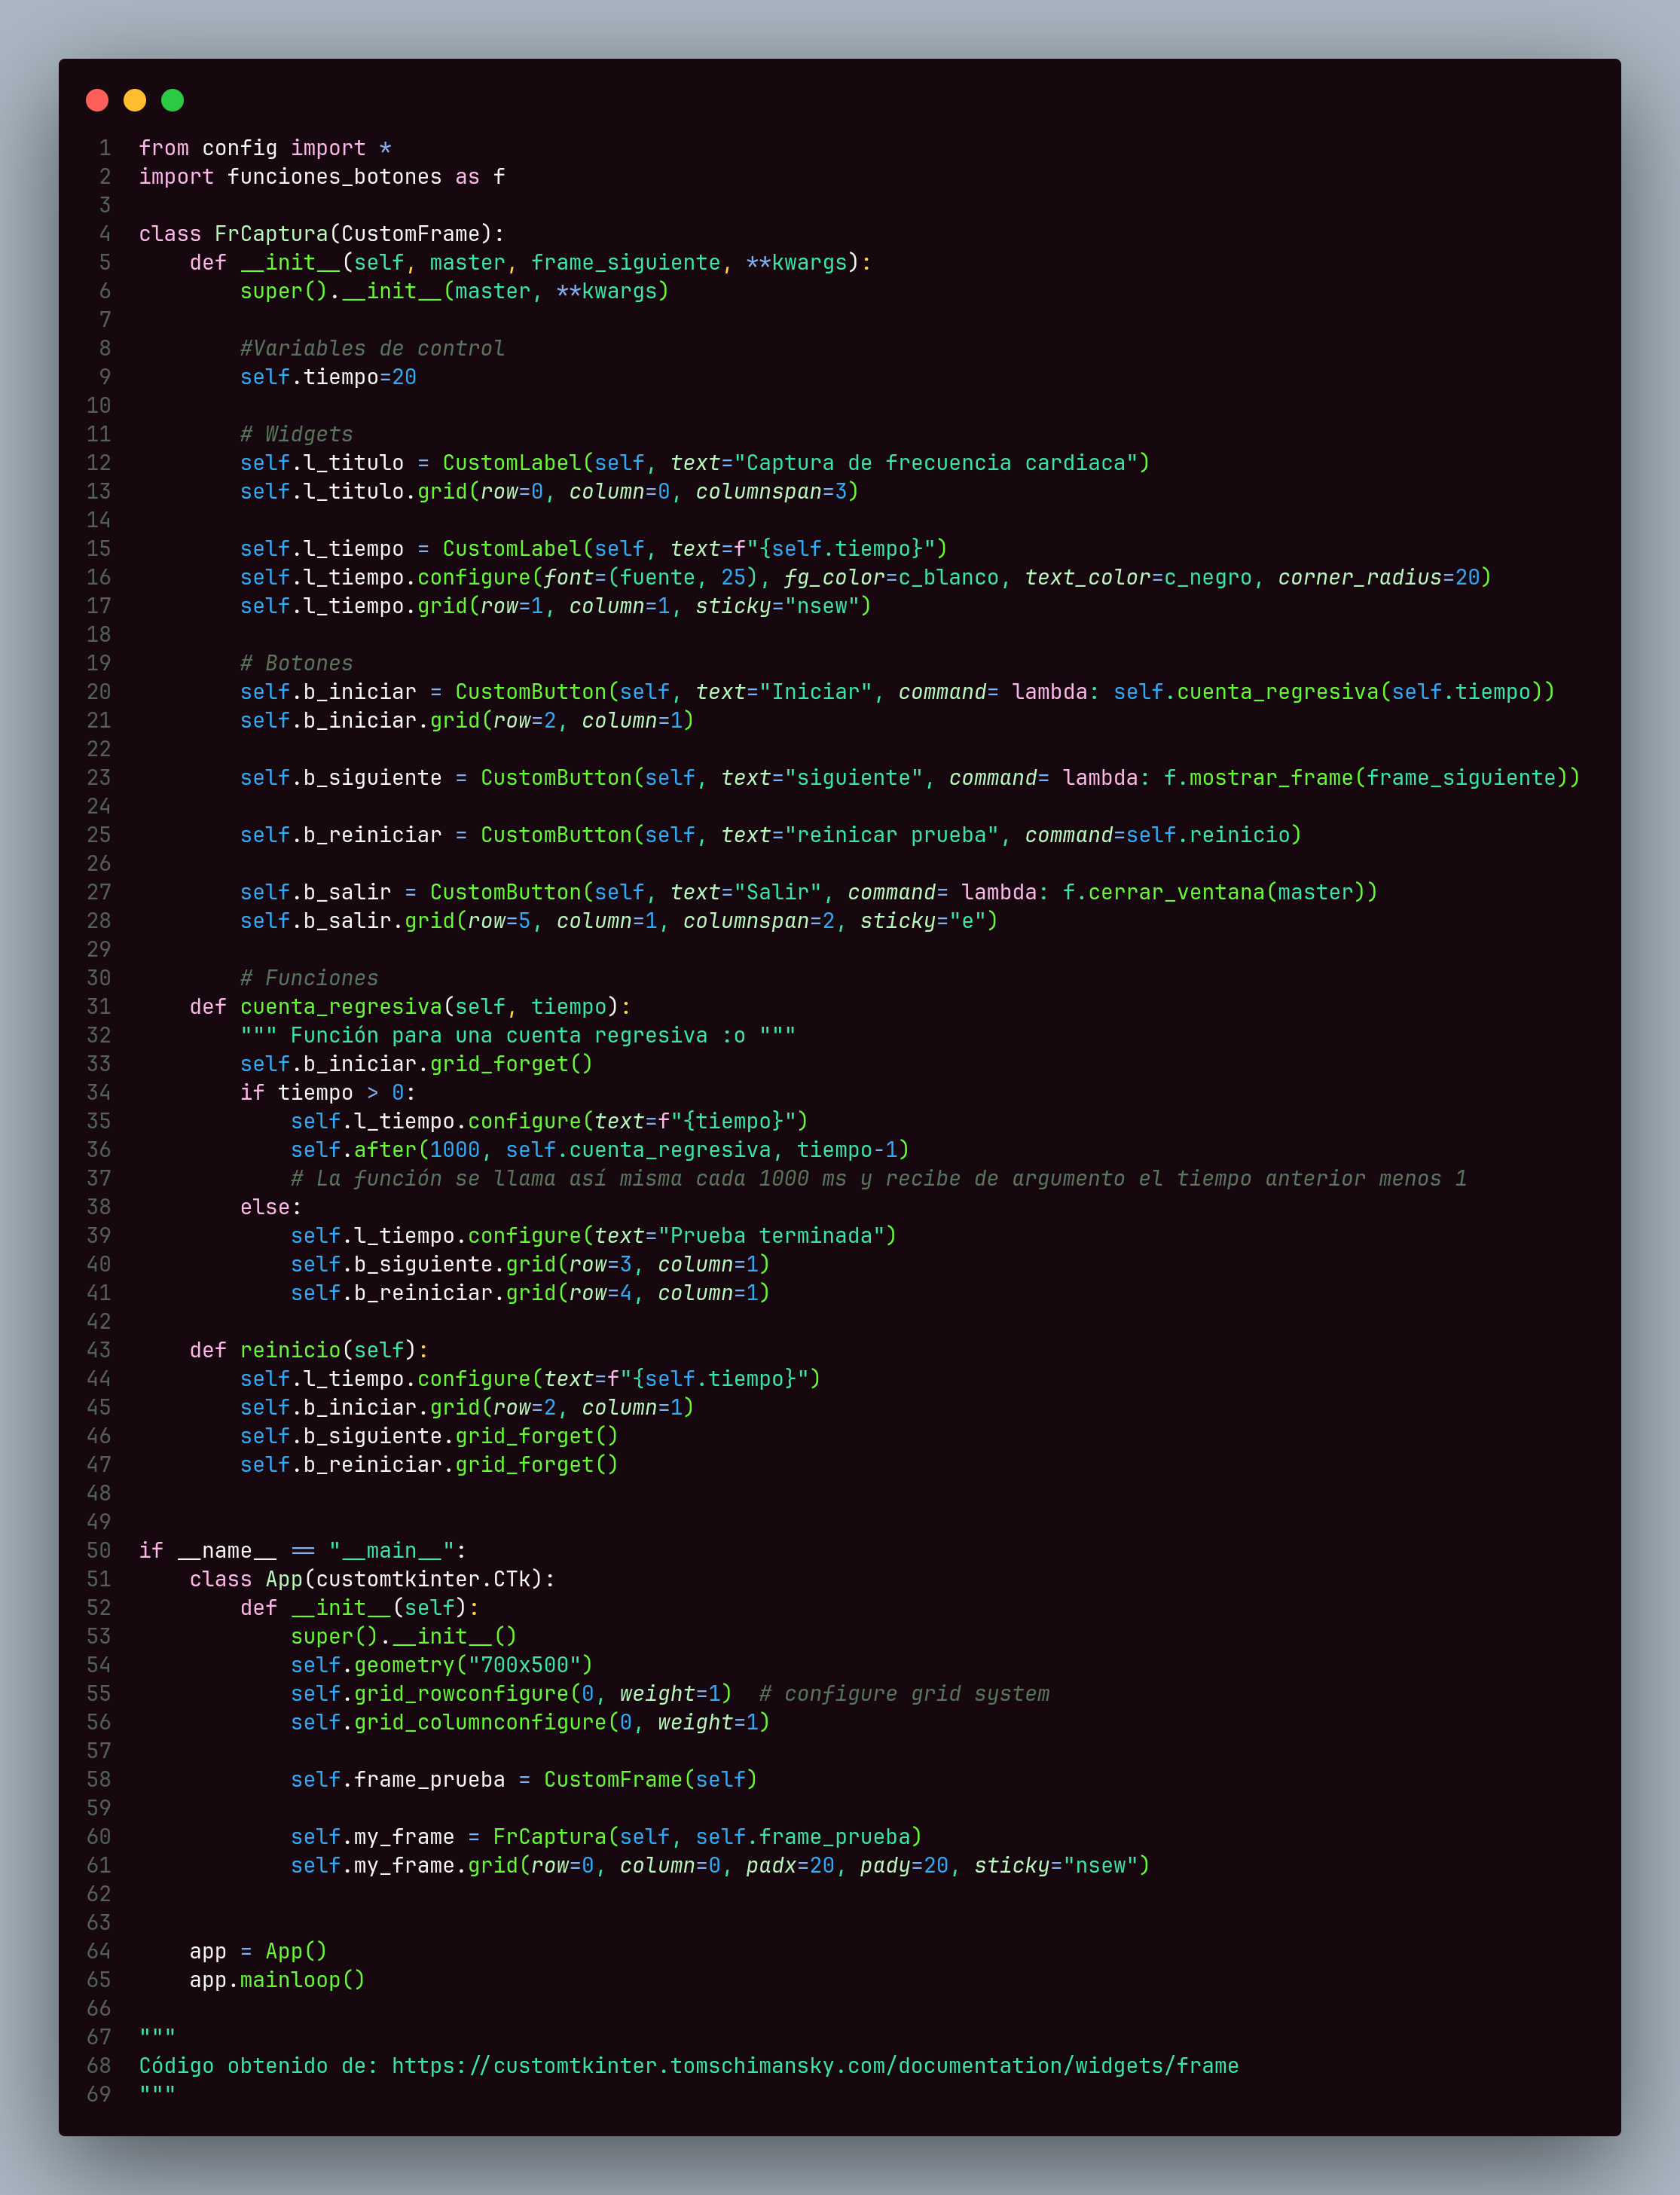
\includegraphics[width=1\textwidth]{pictures/capturas/frames}
	\label{frames}
\end{figure}

\subsubsection{funciones}
En un móulo aparte llamado "funciones botones.py"(figura \ref{funciones}) , se dejaron las funciones más utilizadas por las demás frames a la hora de usar botones, como lo son: mostrar el siguiente frame, cerrar la ventana, etc.

\begin{figure}[h!]
	\caption{Módulo "funciones botones.py}
	\centering
	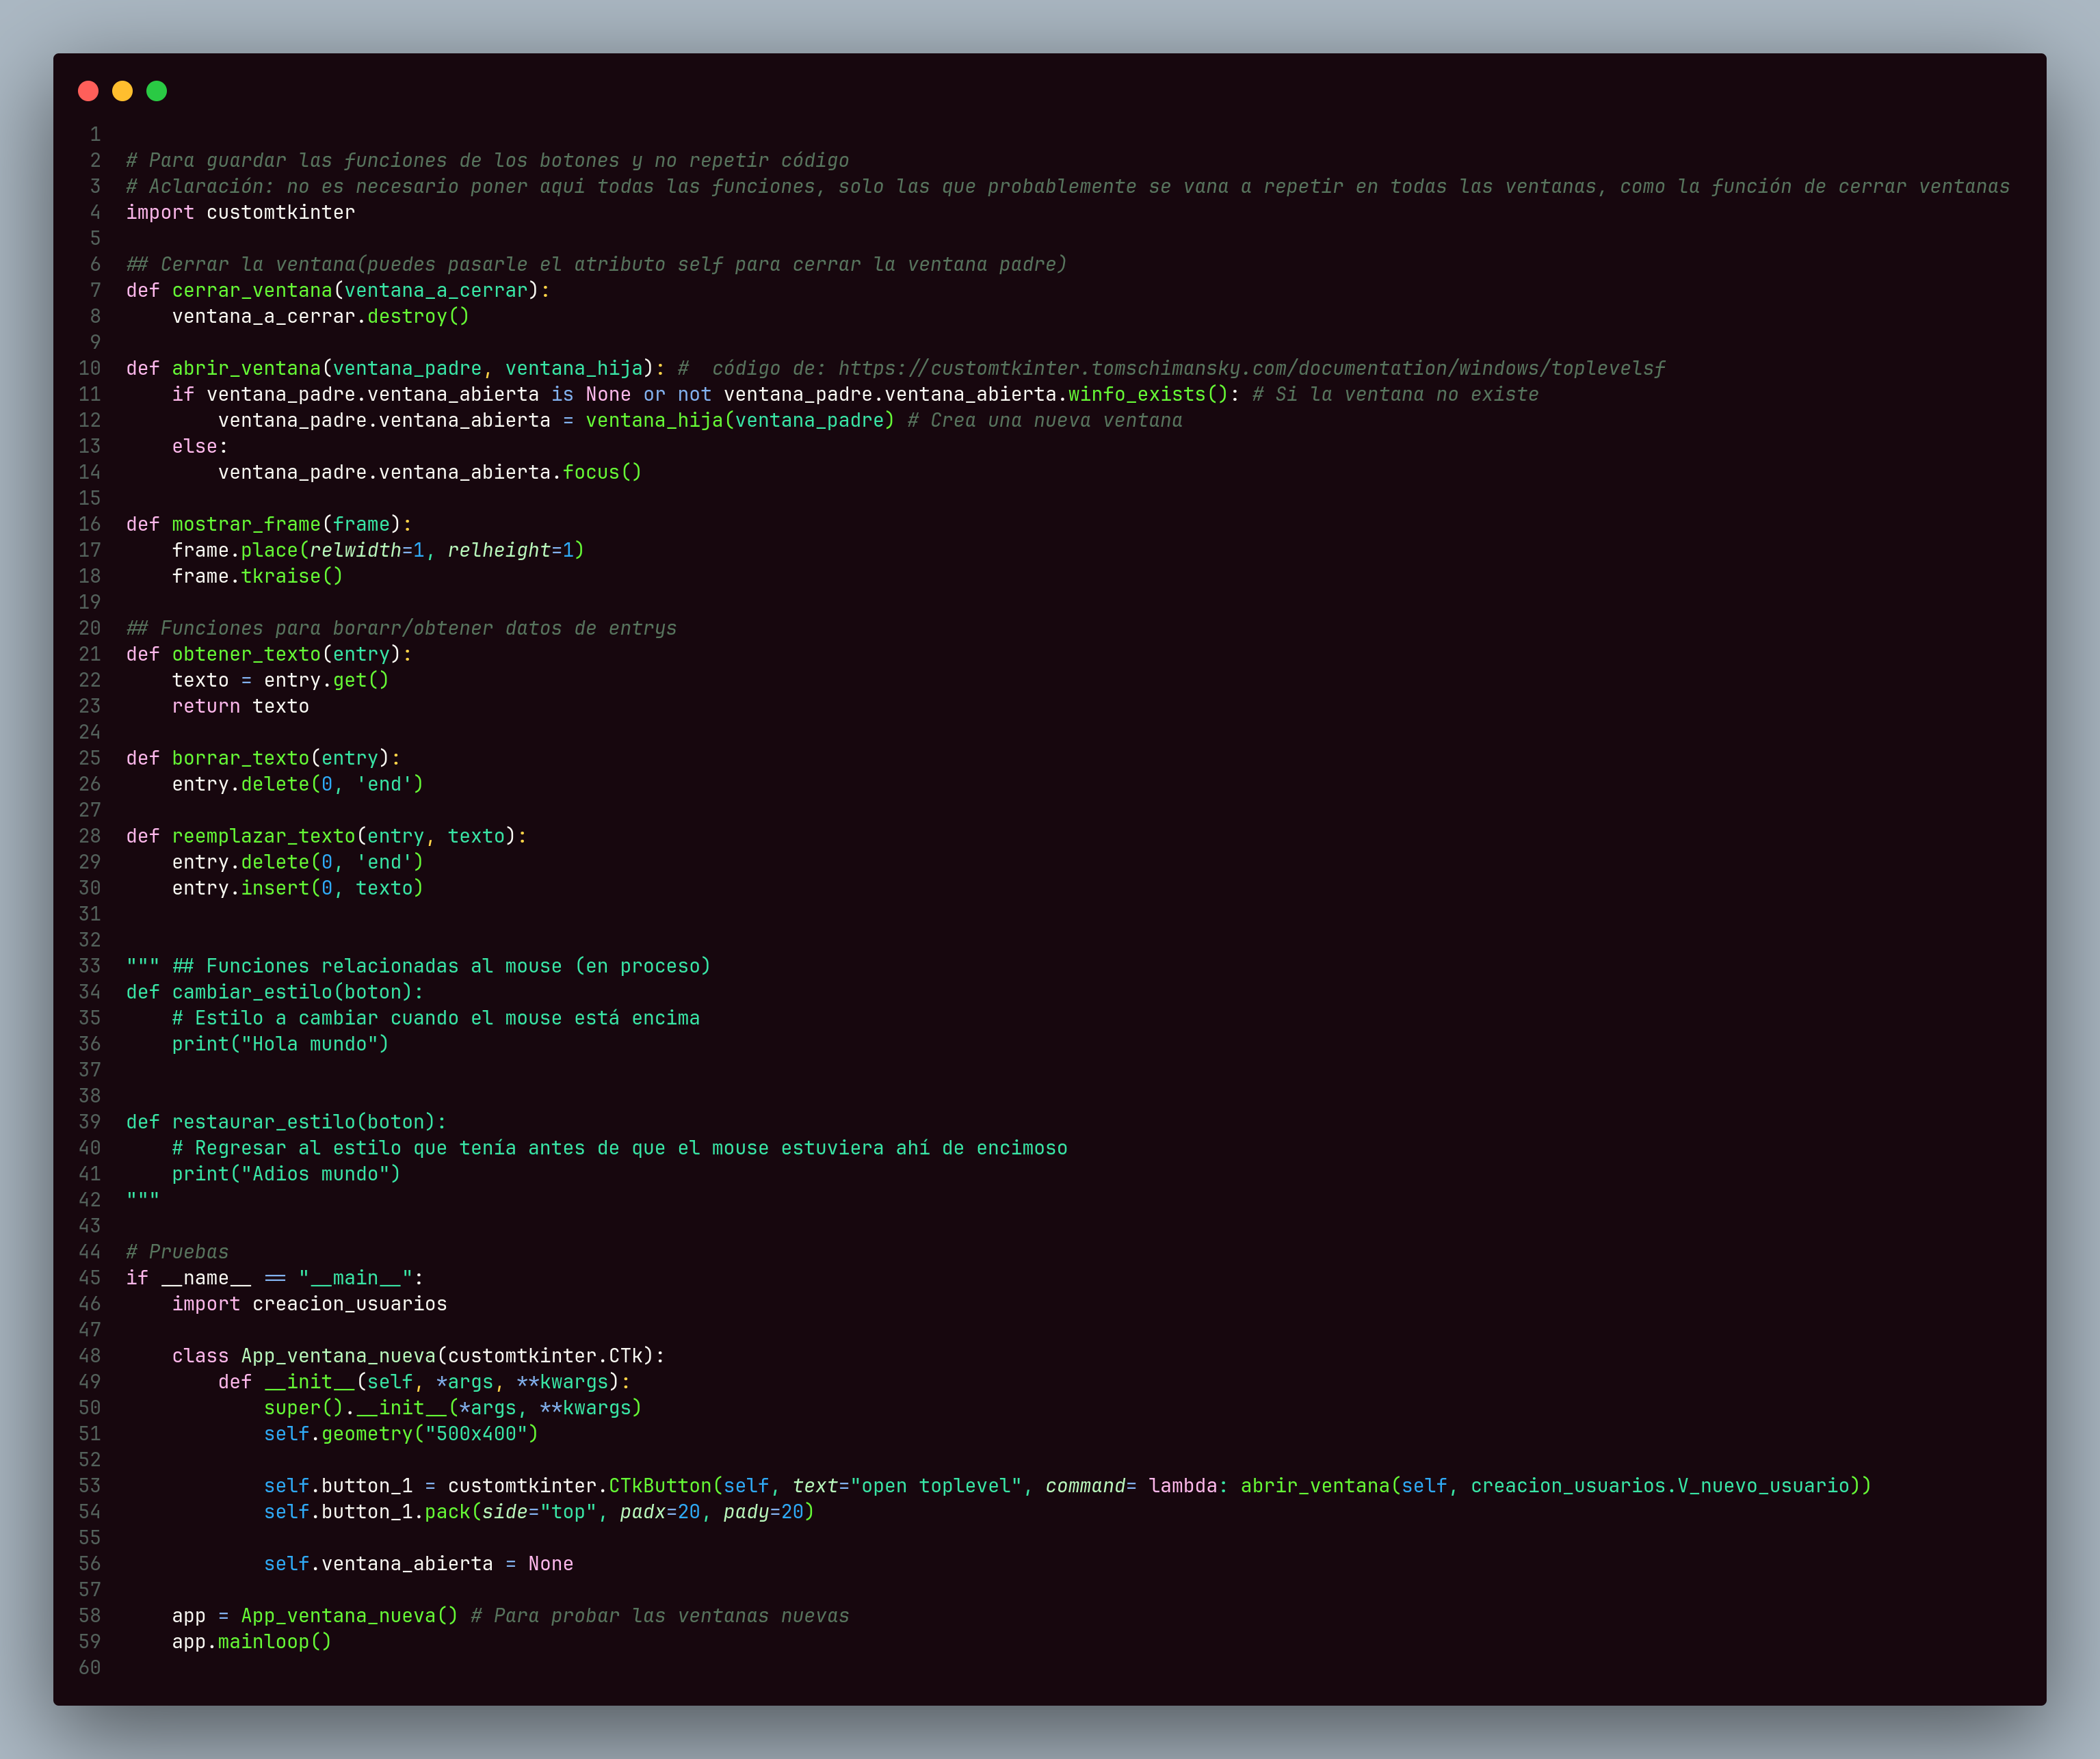
\includegraphics[width=1\textwidth]{pictures/capturas/funciones}
	\label{funciones}
\end{figure}

\subsubsection{ventanas emergentes}
Para la creación de una ventana emergente (figura \ref{ventana}), se siguen los consejos de la documentación de custom tkinter \cite{customtkinter}, donde ya únicamente le agregamos funciones propias de cada ventana y le creamos frames a partir de las clases que previamente hicimos.


\begin{figure}[h!]
	\caption{Ejemplo de creación de una ventana emergente}
	\centering
	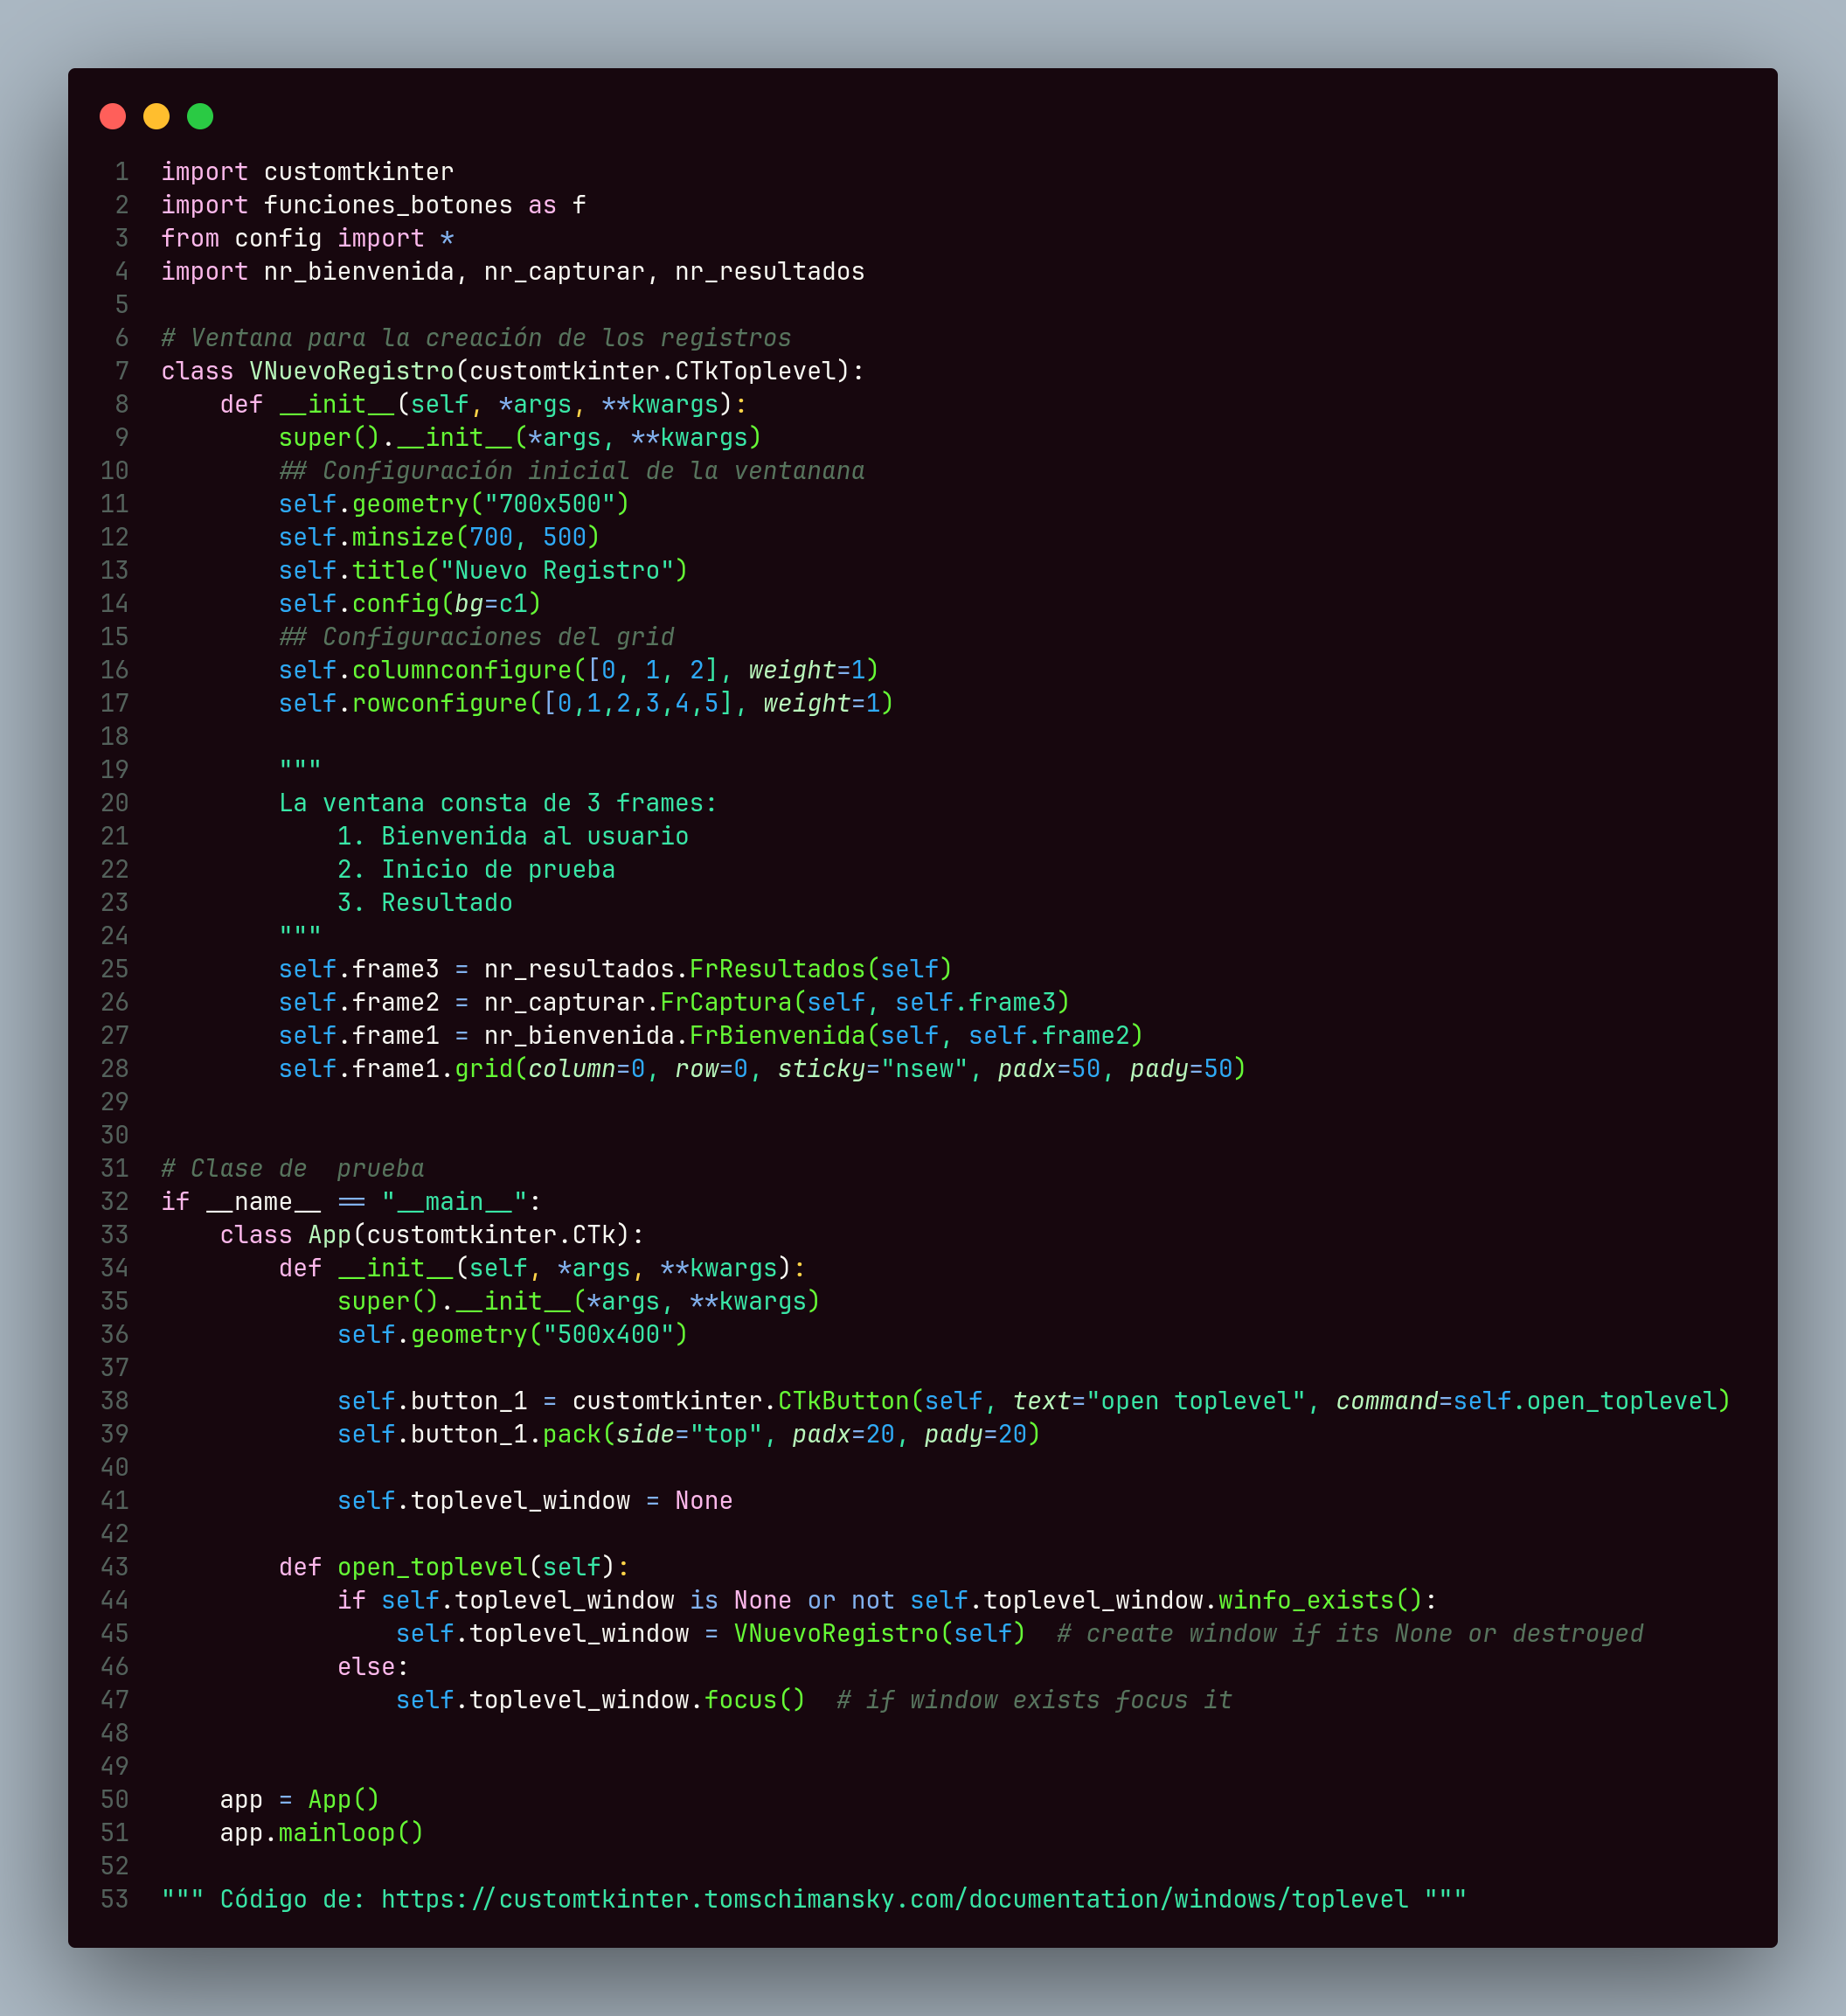
\includegraphics[width=1\textwidth]{pictures/capturas/ventana}
	\label{ventana}
\end{figure}

\subsubsection{Módulo principal}
El módulo principal es el cual se va a ejecutar y llamara como tal a todo el programa, ya listo para usar, en este caso se llama "inicio.py" (figura \ref{inicio})
\begin{figure}[h!]
	\caption{Módulo "inicio.py"}
	\centering
	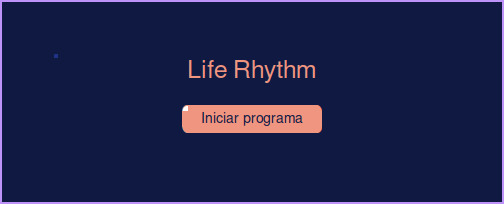
\includegraphics[width=1\textwidth]{pictures/capturas/inicio}
	\label{inicio}
\end{figure}

\subsection{resultados (previos)}
Al ejecutar el módulo principal "inicio.py" (figura \ref{inicio}), se mostrara una imagen con la presentacion del programa (figura \ref{presentacion}), posteriormente tenemos un menú (figura \ref{menu}) en el cual podemos escoger si crear un nuevo usuario o entrar con uno ya creado a partir de su código de usuario. En caso de querer crear un usuario nuevo se abrirá una ventana para poder crear el usuario (figura \ref{nuevousuario}). En caso de haber ingresado con un usuario, llegamos a una ventana principal (figura \ref{vprincipal}) donde puede escoger entre hacer un nuevo registro, hacer una prueba de esfuerzo o graficar los registros que tenga. \\


\begin{figure}[h!]
	\caption{Presentación del programa}
	\centering
	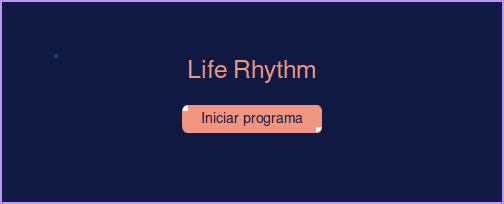
\includegraphics[width=1\textwidth]{pictures/capturas/presentacion}
	\label{presentacion}
\end{figure}

\begin{figure}[h!]
	\caption{Menú que funciona como una especie de "login"}
	\centering
	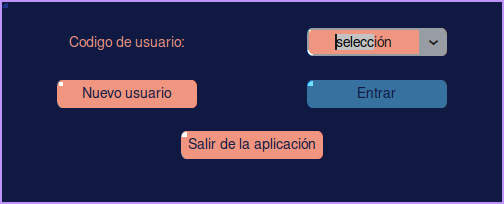
\includegraphics[width=1\textwidth]{pictures/capturas/menu}
	\label{menu}
\end{figure}

\begin{figure}[h!]
	\caption{Ventana para crear un nuevo usuario}
	\centering
	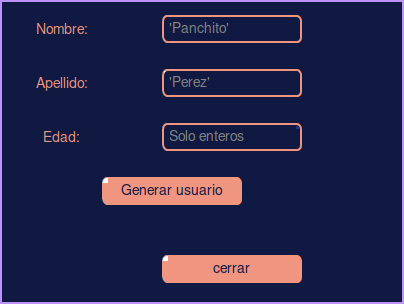
\includegraphics[width=1\textwidth]{pictures/capturas/nuevousuario}
	\label{nuevousuario}
\end{figure}

\begin{figure}[h!]
	\caption{Ventana principal del programa}
	\centering
	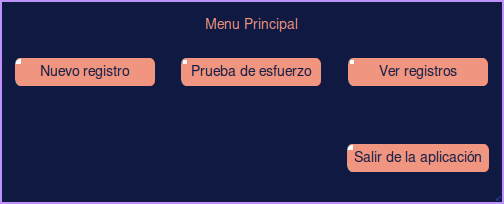
\includegraphics[width=1\textwidth]{pictures/capturas/vprincipal}
	\label{vprincipal}
\end{figure}


\bibliographystyle{plainnat}
\bibliography{referencias2}

\end{document}          
